%
%
%Backscattering in microring resonators
%Guillem Ballesteros
%

%%%%%%%%%%%%%%%%%%%%%%% preamble %%%%%%%%%%%%%%%%%%%%%%%%%%%
\documentclass[10pt,letterpaper]{article}
\usepackage{opex3}
\usepackage{amsmath}

 %\usepackage{ae} %%for Computer Modern fonts

%%%%%%%%%%%%%%%%%%%%%%% begin %%%%%%%%%%%%%%%%%%%%%%%%%%%%%%
\begin{document}

%%%%%%%%%%%%%%%%%% title page information %%%%%%%%%%%%%%%%%%
\title{Characterizing and modeling backscattering in silicon microring resonators}

\author{G. Ballesteros-Garcia, J. Matres, J. Mart\'i and C.J. Oton}

\address{Nanophotonics Technology Center, \\ Universidad Polit\'ecnica de Valencia, Camino de Vera s/n, 46022, Valencia, Spain}

\email{guibalga@ntc.upv.es}


%%%%%%%%%%%%%%%%%%% abstract and OCIS codes %%%%%%%%%%%%%%%%
%% [use \begin{abstract*}...\end{abstract*} if exempt from copyright]

\begin{abstract}
Resonance splitting due to coupling with the counter-propagating mode is the main limiting factor in ring resonators when high-Q factors are required. An experimental method to characterize them together with a theoretical analysis and procedure to extract all the key parameters of the resonator including backscattering is presented.
\end{abstract}

\ocis{(220.0220) Optical design and fabrication; (230.5750) Resonators; (230.3990) Microstructure devices; (250.5300) Photonic Integrated Circuits.}

%%%%%%%%%%%%%%%%%%%%%%% References %%%%%%%%%%%%%%%%%%%%%%%%%
\bibliographystyle{osajnl}
\bibliography{library}

%%%%%%%%%%%%%%%%%%%%%%%%%%%
%%%%%%%%           Introduction           %%%%%%
%%%%%%%%%%%%%%%%%%%%%%%%%%%
\section{Introduction}

Silicon photonics has recently emerged as a viable technology for integrated photonic devices due to the high index contrasts that are achievable and that allow a great confinement of the optical modes. Microring resonators are elements which are simple to fabricate and are used for devices such as optical filters,~\cite{Little1998} sensors,~\cite{DeVos2007} modulators,~\cite{So2004} etc. A high quality factor is usually the key parameter that determines the performance of the device; however, in this technology the factor that limits its highest possible values is in most cases not the propagation loss, which can reach values below 2.4dB/cm~\cite{Dumon2004}, but the backscattering effect due to sidewall roughness~\cite{Morichetti2010a}. Backscattering in a resonator cannot be accounted for as a loss mechanism because in a cavity it can grow coherently much faster than losses. Backscattering is a well known cause of resonance splitting~\cite{Little1997a,Kippenberg2002}; but even before splitting occurs, it can dramatically modify the shape of the resonance, under the right circumstances (under-coupled rings) it can improve the transmission response by pulling down on the resonance making it look as if the ring is nearer to the critical coupling condition. If this effect is not taken into account and one extracts the parameters of the ring from a fit, it can produce a good curve agreement but with very wrong results.  In this paper, we propose a characterization technique and a fully analytical fitting procedure that allows a complete characterization of all the parameters of the ring including backscattering, without the need of a coherent backscattering measuring system as in~\cite{Morichetti2010a,Morichetti2010b}.

%%%%%%%%%%%%%%%%%%%%%%%%%%
%%%%%%     Experiment      %%%%%%%%%%%
%%%%%%%%%%%%%%%%%%%%%%%%%%
\section{Experiment}

Silicon waveguides were fabricated from silicon-on-insulator (SOI) wafers with 220nm Si thickness and 2$\mu$m buried oxide thickness. Waveguides are fully-etched 220$\times$450nm channels which are covered with a 2$\mu$m $SiO_2$ layer, and grating couplers were used for coupling the light from standard single-mode fibers at $10^o$ angle. Waveguides and gratings were both patterned with deep-UV lithography. Transverse-electric (TE) polarization was used in all the experiments. Transmission spectra were collected with a tunable laser with 1~pm resolution with 2~dBm input power in fiber. The rings had a 20$\mu$m radius and two coupling points, providing a \emph{through} and a  \emph{drop} port. However, in this experiment we also collect the counter-propagating drop port, which we will call \emph{counter-drop} port. Measuring this port is crucial to fully characterize the ring, as it directly provides the information about the backscattering inside the cavity. The gap of the through and drop couplers was 275nm and 300nm respectively. 
%%%%%%%%%%%%%%%
\begin{figure}
    \centering
    \includegraphics[height=4.5cm]{add_drop_ring.eps}
    \caption{Proposed layout for future add-drop rings with drop (D), counter-drop (CD) and through (T) ports.}
    \label{fig:add_drop_ring}
\end{figure}
%%%%%%%%%%%%%%%%%%

Figure~\ref{fig:espectro} shows the measured transmission through all three ports of one microring. It is worth noting that the shape of the resonances is very variable, even though one would expect the loss and the coupling coefficients to be approximately the same in all cases. The reason for this behavior is the backscattering parameter, which is intrinsically noisy, thus producing an apparently random response in their resonances. It is noisy because reflections are produced by sidewall roughness along the ring, so they are randomly distributed along its length, and the overall reflection coefficient results from the interference of all the components, giving rise to sharp spectral variations. In order to extract the parameters of the ring, one must take into account backreflection, otherwise the estimation of the loss and coupling coefficients would depend on which resonance we select, which is unphysical and would produce wrong results. Therefore, a procedure to extract all the parameters including backreflection is needed in order to understand the behavior of our microring resonator. Next section provides an analytical treatment and a recipe to extract all the parameters from any given resonance.

%%%%%%%%%%%%%%%%%%%%%%%%%%%%%%%%%%%%%%%
\begin{figure*}[t]
    \centering
    \includegraphics[width=1.0\textwidth]{grafica_opexe.eps}
    \caption{Top panel: Transmission spectrum of each port of the microring: the \emph{through} (red, solid), the \emph{drop} (blue, dashed), and the \emph{counter-drop} (green, dash-dot). Bottom panels: Detail of the 3 resonances labeled $a$, $b$ and $c$ corresponding to peaks at 1549, 1553 and 1558~nm, where frequency and transmission have been normalized. Solid curves are the experimental data and dashed lines are the analytical curves using the parameters extracted from the fitting procedure and shown on top of each peak in the second row.}

    \label{fig:espectro}

\end{figure*}
%%%%%%%%%%%%%%%%%%%%%%%%%%%%%%%%%%%%%%%


%%%%%%%%%%%%%%%%%%%%%%%%%%%
%%%%%%%%%%         Theory     %%%%%%%%%
%%%%%%%%%%%%%%%%%%%%%%%%%%%
\section{Theory}
\label{sec:theory}

A method for coupled resonators in the time-domain~\cite{Haus1984} was used to describe the ring, since it has already been proven to work for ring resonators where the propagating and counter-propagating modes are coupled through a coupling constant~\cite{Zhang2008}.
Typically time-domain analyses take the photon life times as parameters, but these can be readily related to the usual energy coupling and losses constants of a space-domain analysis~\cite{J.HeebnerR.Grover2008} as in~\cite{Little1997} by:

\begin{equation}
    K_j=\frac{\omega_oL}{Q_{e,j} v_g}  \qquad \alpha=\frac{\omega_o}{Q_i v_g} \qquad \sqrt{R}=\frac{\omega_oL}{2Q_rv_g}
\label{eq:space-constants}
\end{equation}

where the Q-factors are related to the $\tau$ constants of the time domain-model through $Q_j=\omega_o \tau_j/2$. The Q-factors $Q_{e,1}$, $Q_{e,2}$, $Q_{i}$ and $Q_{r}$ correspond respectively to the coupling with the bottom and top waveguides, the intrinsic losses and the coupling constant; $v_g$ is the group velocity of the waveguide and can be obtained from the free spectral range (FSR) of the ring. Finally, $Q_r$, has been related to the total reflectivity in a single-pass, that is, the fraction of energy coupled into the counter-propagating mode in one trip around the ring. Although the characteristics of the model imply a uniformly distributed backscattering, reflections really occur at randomly localized points, giving rise to the random nature of the variations of backscattering versus wavelength~\cite{Morichetti2010}. The quality factor of the whole system is defined in the usual way as:

\begin{equation}
	    \frac{1}{Q}=\frac{1}{Q_{e,1}}+\frac{1}{Q_{e,2}}+\frac{1}{Q_i}
\end{equation}

Following the guidelines in~\cite{Haus1984,Little1997,Zhang2008} the expressions for the signal in the different ports shown in Fig.~\ref{fig:add_drop_ring} are easily expressed in terms of quality factors as:
\begin{align}
	T=& \left\lVert1-\frac{        \frac{2}{Q_{e,1}}(2j(\omega '-1)+\frac{1}{Q})   }  {   (2j(\omega '-1)+\frac{1}{Q})^2+\frac{1}{Q_r^2}  }\right\rVert^2 \label{eq:T} \\
	D =& \left\lVert\frac{          \frac{2}{\sqrt{Q_{e,1}Q_{e,2}}}(2j(\omega '-1)+\frac{1}{Q})   }  {   (2j(\omega'-1)+\frac{1}{Q})^2+\frac{1}{Q_r^2}    }\right\rVert^2 \label{eq:D} \\
	C=& \left\lVert\frac{          \frac{2}{Q_r\sqrt{Q_{e,1}Q_{e,2}}}   }  {   (2j(\omega'-1)+\frac{1}{Q})^2+\frac{1}{Q_r^2}    }\right\rVert^2 \label{eq:CD}
\end{align}

where $\omega'$ is the normalized angular frequency of the resonance under study.

In order to extract the value of the different parameters, a measurement of the through, drop and counter-drop ports is needed. After solving the expressions that result from particularizing equations~\ref{eq:T},\ref{eq:D}, \ref{eq:CD} for $\omega'=1$  ($T_o,D_o,C_o$) and calculating the normalized width ($\Delta\omega'$) of the counter-drop port defined from $C(\omega'=1\pm\Delta\omega'/2)=C_o/2$ the quality factors can be expressed as:

\begin{align}
    Q=&\frac{1}{\Delta\omega'}\left(\frac{C_o}{D_o}-1 + \sqrt{2}\sqrt{\left(\frac{C_o}{D_o}\right)^2+1}\right)^{1/2} \label{eq:Q} \\
    Q_r=&\frac{1}{Q}\sqrt{\frac{D_o}{C_o}} \label{eq:Qu}\\
    Q_{e,1}=&\frac{2}{Q(Q^{-2}+Q_r^{-2})(1\pm\sqrt{T_o})}  \label{eq:Qe1}\\
    Q_{e,2}=&\frac{2(1\pm\sqrt{T_o})}{QD_o(Q^{-2}+Q_r^{-2})}  \label{eq:Qe2}
\end{align}

In eq.~\ref{eq:Q}, $\Delta\omega'$ is equivalent to the half-width at half maximum only when there is no splittin in the counter drop signal. The 4 parameters that characterize the ring in a space-domain formalism can be calculated using eq.~\ref{eq:space-constants}. The sign ambiguity in equations~\ref{eq:Qe1} and \ref{eq:Qe2} is a byproduct of the existence of two degenerate operation regimes in the ring with different parameters but the same resonance shape. This ambiguity is well known in cases without any backreflection effect, and it is usually  overcome by measuring rings with different parameters or looking at the dependence on wavelength as in \cite{McKinnon2009}. In our case, the ambiguity only occurs for the peak with lowest reflection coefficient (the peak labeled as (b)), as in the other two cases it would give rise to a negative loss coefficient, which is unphysical, because it requires gain from the medium. As the sign has to be the same in all the peaks of the same ring, this provides a way to decide the correct sign in the expressions by analyzing more than one peak and looking for non-physical solutions.

After some numerical simulations one finds that there 3 main regimes of operations in which the ring can work. They are distinguished by how strong is the coupling in relation to the other mechanisms, that is, how big is $Q_r$ in comparison with $Q$. In first place, when $Q_r \gg Q$, the coupling can be considered to be negligible and the parameters can be extracted with already existing methods like in~\cite{McKinnon2009}, or by doing $1/Q_r=0$ in eq.~\ref{eq:T} and solving for $Q_{e,1}$ and $Q$ as a function of the extinction ratio and the half-width at half depth. In this situation all resonances tend to have approximately the same shape and don't show splitting. If the interest is in achieving high quality factors then the usual regime of operation is $Q_r \sim Q$ and the expressions described in this paper should be used. Nevertheless, it may not be obvious from a measurement of the through port that the latter is the actual mode of operation since resonances don't always split, under this circumstances one should look at the different peaks and see if they vary in an apparently random fashion, and where possible the counter drop port response. If the coupling is strong, $Q_r \ll Q$, which may happen if the rings are intentionally designed for this purpose, then simplified expressions can be found (see table~\ref{tab:summary}). If this is the case then splitting is very evident showing two clearly defined peaks around each resonance frequency.

%%%%%%%%%%%%%%%%%%%%%%
%%%%%%        Results        %%%%%%%
%%%%%%%%%%%%%%%%%%%%%%

\section{Results}
%The measured spectra at the three ports can be seen in Fig.~\ref{fig:espectro}. As it is expected from the results in \cite{stat_backscattering}, the extinction ratios and characteristics of the different resonances show a great variability since the backscattering differs from one resonance to the next. This effect can only be observed at high Q-factors due to the increasing relative importance of $Q_u$ with respect to $Q$.

From the experimental data shown in Fig.~\ref{fig:espectro}, we have chosen three consecutive resonances which show quite different behavior in terms of extinction ratio and degree of splitting. The results obtained from the method described in section~\ref{sec:theory} for each resonance are also shown in Fig.~\ref{fig:espectro}, and the corresponding theoretical curves are shown in the insets, where a good agreement is observed. It is worth noting that the coupling constants and the loss show small variations among resonances, being $R$ the one showing the strongest variations. This is expected from the nature of backscattering, and is a demonstration of the validity of our model. The asymmetry of the shape of peaks 1 and 3, which is not reproduced in the theory, could be explained by sudden variations in the reflection coefficient along the width of the resonance, which is not considered in the model.


%%%%%%%%%%%%%%%%%%%%
%%%%%    Conclusion     %%%%%%%
%%%%%%%%%%%%%%%%%%%%

%%%%%%%%%%%%%%%%%%
%%Tabla resumen

\begin{table}[ht]
	\renewcommand{\arraystretch}{1.3}
	\caption{Summary of expressions for calculating Q-factors of ring-resonators working under different backscattering regimes}
	\centering
	\begin{tabular}{ccccc}
	\hline
	Weak coupling && Intermediate coupling && Strong coupling\\
	$(Q_r \gg Q)$ && $(Q_r \sim Q)$ && $(Q_r \ll Q)$\\
	\cline{1-1} \cline{3-3} \cline{5-5}
	$Q=1/\Delta\omega'_{\mbox{\scriptsize{FWHM}},D}\footnotemark[1]$&&$Q$ (eq.~\ref{eq:Q})&&$Q=1/\Delta\omega'_{FWHM}$\\
	$Q_r$ (eq.~\ref{eq:Qu})&&$Q_r$ (eq.~\ref{eq:Qu})&&$Q_r=1/splitting\footnotemark[2]$\\
	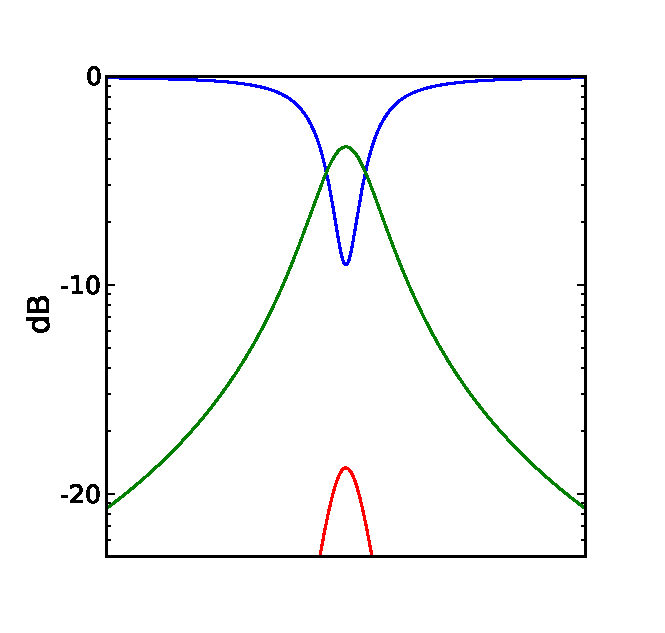
\includegraphics[scale=0.4]{graphic0.eps}&&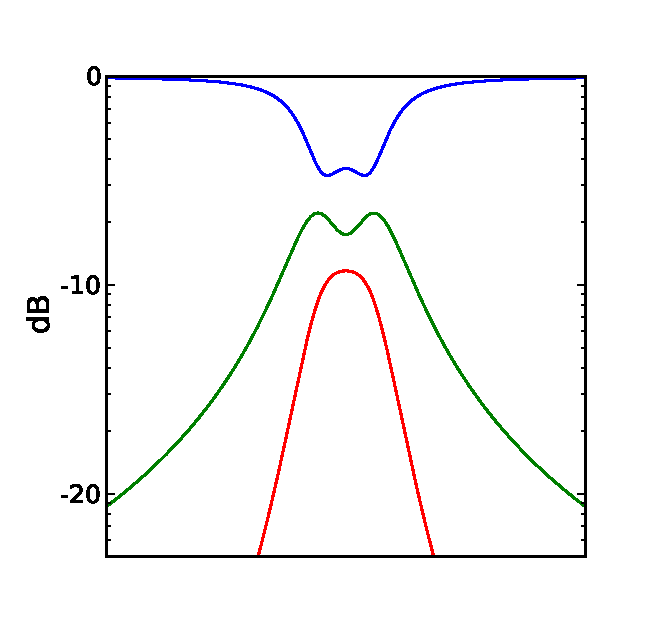
\includegraphics[scale=0.4]{graphic1.eps}&&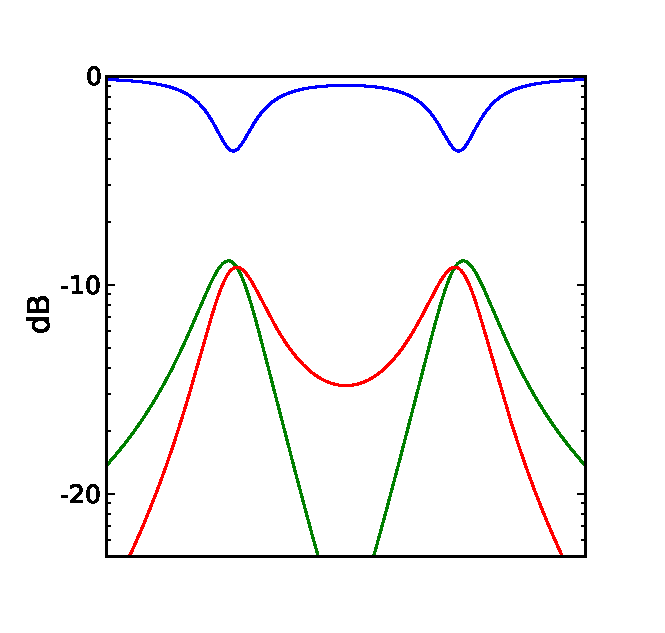
\includegraphics[scale=0.4]{graphic2.eps}\\
	\hline
	\multicolumn{4}{l}{\footnotemark[1]{\footnotesize{Full-width at half maximum of the drop port}}}  \\
	\multicolumn{2}{l}{\footnotemark[2]{\footnotesize{Peak to peak distance}}}
	\end{tabular}
	\label{tab:summary}

\end{table}%
%%%%%%%%%%%%%%%%%%%%%%%%


\section{Conclusion}
We have described an analytical model and a fitting procedure that allows extraction of all the key parameters of a silicon microring resonator with two coupling points. These parameters are both coupling constants, propagation loss and the backscattering coefficient. With this method, we demonstrate that variations of the backscattering parameter are the cause of the strong variations in the shape of different resonances of the same microring. All these parameters can be extracted from simple transmission measurements using a standard characterization setup.

%We think that the methods described in this paper to analyze the parameters from a ring-type resonator when high-Q factors are intended, is an improvement with respect to other methods that don't take into consideration the effects of mutual mode coupling due to backscattering in the ring. Our method also allows for a way to measure the backscattering in waveguides with a standard characterization setup.
%\setlength{\textfloatsep}{7pt} 



\section*{Acknowledgments}


The authors acknowledge financial support from the Spanish Ministry of Science and Innovation through contract SINADEC (TEC2008-06333). EPIXfab is also acknowledged for the fabrication of the devices.

\end{document} 
